\section{I курс}

\AddProb К висящей очень лёгкой пружине жёсткостью $k$ подвешен шарик. Вначале пружина 
не растянута. Затем шарик отпускают. Какой максимальной скорости достигнет шарик 
при своем движении? Масса шарика $m$.

\AddProb Если смотреть на свет сквозь две гребёнки с разной частотой зубьев, наложенные 
друг на друга, то светлые участки будут чередоваться с тёмными. С какой скоростью 
будут перемещаться эти участки, если одну из гребёнок двигать относительно второй со 
скоростью 1 см/с? Неподвижная гребёнка имеет 5 зубьев и 5 промежутков между ними на 
сантиметр, а движущаяся~--~6.

% Задача (82) Энергия и импульс
\begin{wrapfigure}{r}{4cm}
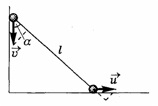
\includegraphics[width=4cm]{0611EnergyAndImpulseBar.jpg}
\end{wrapfigure}

\AddProb Два тела малых размеров массой $m$ каждое соединены стержнем пренебрежимо малой массы длиной $l$. 
Система из начального положения у вертикальной гладкой стены приходит в движение. 
Нижнее тело скользит без трения по горизонтальной поверхности, верхнее - по вертикальной. 
Найдите значение скорости нижнего тела, при котором верхнее оторвется от вертикальной стенки.


\section{II курс}

\AddProb Если смотреть на свет сквозь две гребёнки с разной частотой зубьев, наложенные 
друг на друга, то светлые участки будут чередоваться с тёмными. С какой скоростью 
будут перемещаться эти участки, если одну из гребёнок двигать относительно второй со 
скоростью 1 см/с? Неподвижная гребёнка имеет 5 зубьев и 5 промежутков между ними на 
сантиметр, а движущаяся~--~6.

\AddProb Найдите частоту колебаний полярной молекулы в однородном электрическом поле, напряженность которого $E$\,=\,300~В/см. 
Полярную молекулу можно представить в виде жесткой гантельки длины $l\,=\,10^{-8}$~см, на концах которой находятся две материальные точки 
массы $m\,=\,10^{-24}$~г, несущие на себе заряды $e\,=\,1.6\times10^{-24}$~Кл и $-e$ соответственно. 

\AddProb Для определения отношения теплоёмкостей газа при постоянном давлении и при 
постоянном объёме иногда применяется следующий метод. Определённое количество газа, 
начальные объём и давление которого равны соответственно $V_0$ и $p_0$, нагревают 
платиновой проволокой, через которую в течение определённого времени проходит 
электрический ток: один раз при постоянном объёме $V_0$, причём газ достигает давления $p_1$, 
другой раз при постоянном давлении $p_0$, причём объём газа становится равным $V_1$. Как, 
измеряя эти величины, определить отношение теплоемкостей?


\section{III и IV курсы}

\AddProb Шар-зонд, имеющий нерастяжимую оболочку, поднялся на максимальную высоту и совершает малые колебания около равновесного уровня. 
Найдите период этих колебаний, считая, что на такой высоте плотность воздуха $\rho$ убывает с высотой равномерно на величину 
$\delta\,=\,1.2\times10^{-2}\,\rho$ через каждые $h$~=~100~м. Трением шара о воздух пренебречь.

\AddProb Однородно заряженный куб создаёт в своей вершине~$A$ электрическое поле напряжённостью~$E$. Из куба удалили кубик вдвое 
меньших размеров. Чему теперь будет равна напряжённость поля в точке~$A$?

\AddProb Оцените, за какое время застынет лед средней толщины $D$~=~0.5~м на озере во время холодной зимы. Считайте, что теплопроводность льда 
$\kappa$~=~2.2 Вт/(м$\cdot\,$К), удельная теплота кристаллизации $q\,=\,3.4\times10^5$ Дж/кг, плотность $\rho\,=\, 0.9\times10^3$ кг/м$^3$. 
Принять, что внешняя температура постоянна и равна $T_0\approx263$~К. 